\documentclass{article}
\usepackage[utf8]{inputenc}
\usepackage{float}

\title{\textbf{Preliminary Research Proposal}\\Investigating the Microscopic Mechanics of Hair-Hydrometer and mechanical properties of keratin fibrils via Atomic Force Microscopy }
\author{Jun-Yan Zhang}

\date{August 2019}

\usepackage{natbib}
\usepackage{graphicx}
\usepackage{amsmath}

\begin{document}

\maketitle


\section{Topic}
\begin{itemize}
\item What's the microscopic mechanism of the Hair-Hydrometer?
\item How a normal kerotin in human hair change in morphology and its Young's Modulus with the change of environment humidity and temperature? 
\item What's the relationship between the kerotin's mechanical properties and the macroscopic mechanical properties of human hair?
\end{itemize}

\section{Background}
A simple hygrometer can be built stretching a bunch of degreased human hair, invented in 1800 by a swiss physicist and the founder of mountaineering, de Saussure. Even now the hair-hydrometer is still playing an important role in meteorological oservatories all over the world because its high precision. 

The Young's modulus (YM)  of the hair(usually around $2\mathrm{Gpa}$) will change with the humidity, temperature and other factors of the environment and thus the hair length will change under a fixed tension applied at two endings of the hair. The previous work done by our team found out the rough relation between hair length and environment factors in a macroscopic view, and we hypothised a physical model to explain the phenomenon using estimated density of Hydrogen bonds between kerotins, which is the core compounds consisting human hair and the chemical equilibrium of Hydrogen bond breaking under different humidity and temperature (hydrogen bonds provide a part of the hair's stiffness), but the microscopic mechanics is still under debating.

Enlightened by the Atomic Force Microscopic(AFM) imaging for Young's Modulus(YM) of amyloid fibrils \citep{lee2016advances}(they used an advanced AFM mode, Peak Force Quantitative Nanomechanics Measurement (Peak Force QNM) mode, to get the \textbf{radial} YM data of amyloid fibrils under different conditions (e.g., in different environment, after different incubation time) by nano-indentation), we came up an idea that to make kerotins fibrils as the specimen instead of amyloid fibrils.  \\
We can control the environment easily by setting up the whole instrument in a artificial box allowing us to adjust the humidity and the temperature.

\subsection{Literature review}
At beginning (1921), people thought it was humidity that changes the curvature of water menisci in the hair cell pores and then strain or loosen the cell walls. The mechanical properties of hair follows Hooke's law\citep{Whipple_1921}.
\begin{figure}[H]
    \centering
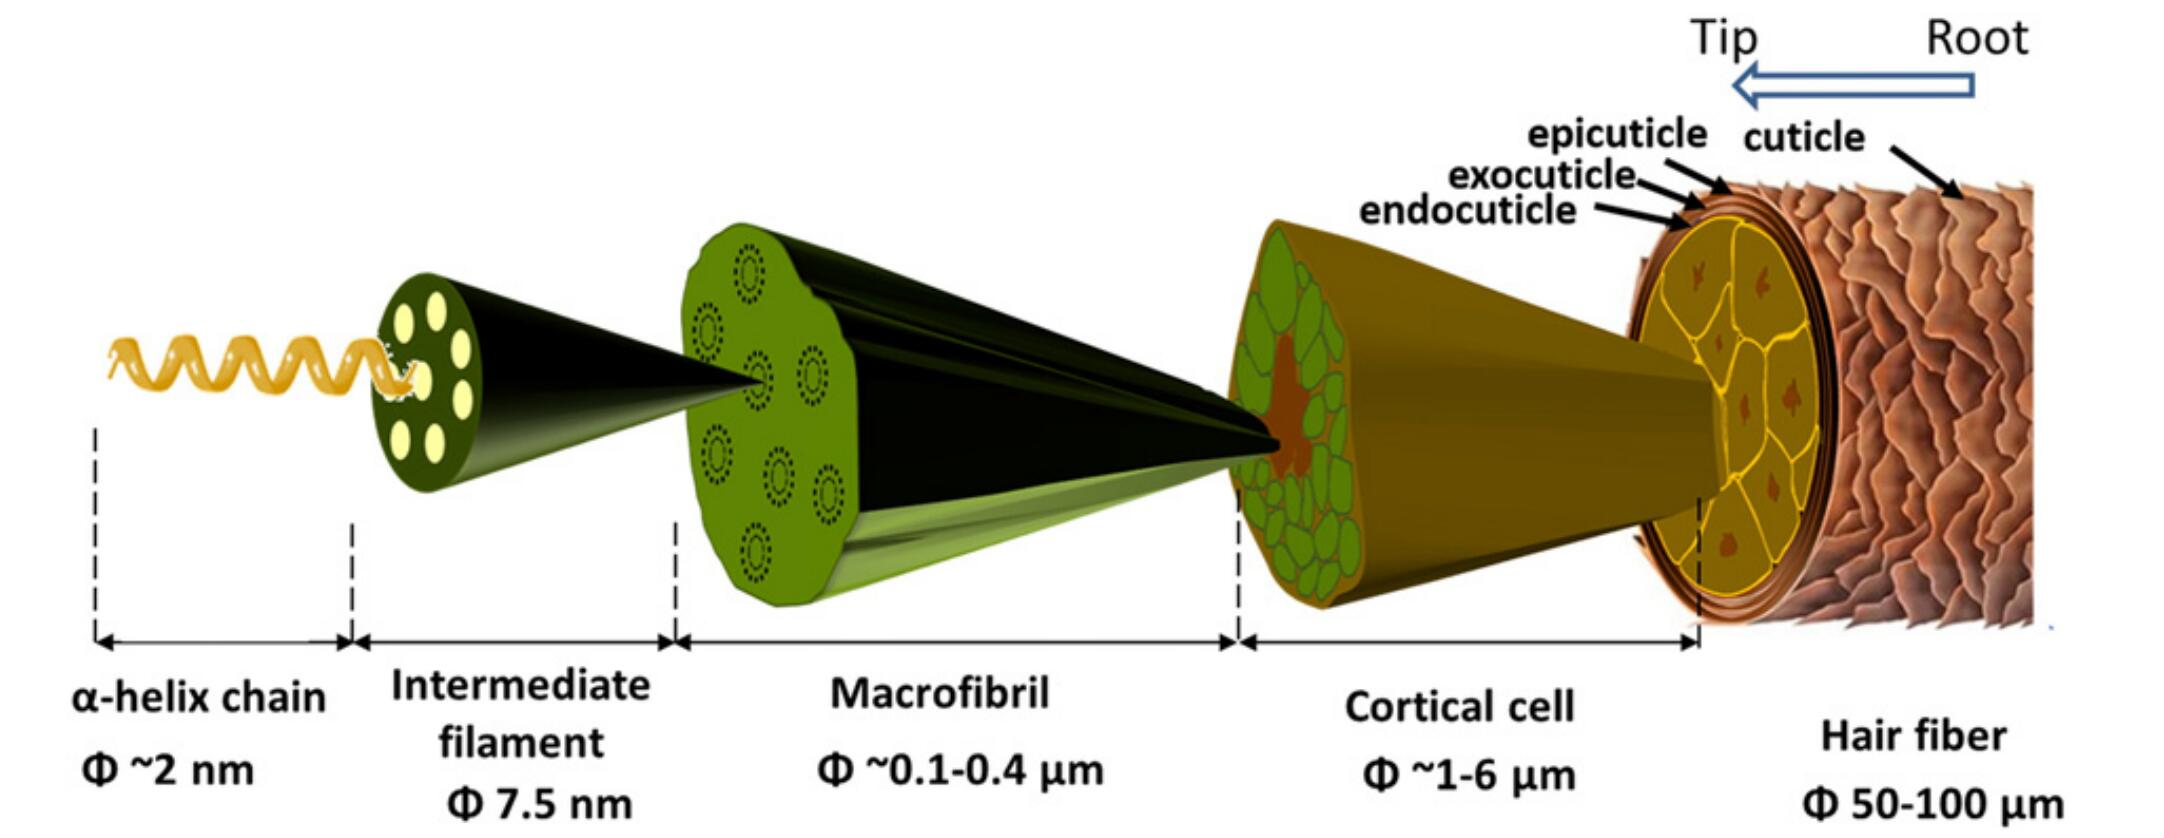
\includegraphics[width=0.85\textwidth]{hair structure.jpg}
    \caption{hair structure\citep{yu2017structure}}
\end{figure}
Human Hair is mainly consisted by curtail, cortex, and medulla from outside to the center, and cortical cell are mainly formed by  keratin fibrils (alpha).

Till now, many efforts have been spend to under stand the link between keratin fibrils and hair's mechanical properties.


 In \citep{yu2017structure}, they used $\alpha$ and $\beta$ kerotin model (examined by X-ray scattering) to explain the elasticity of human hair:
\begin{figure}[H]
    \centering
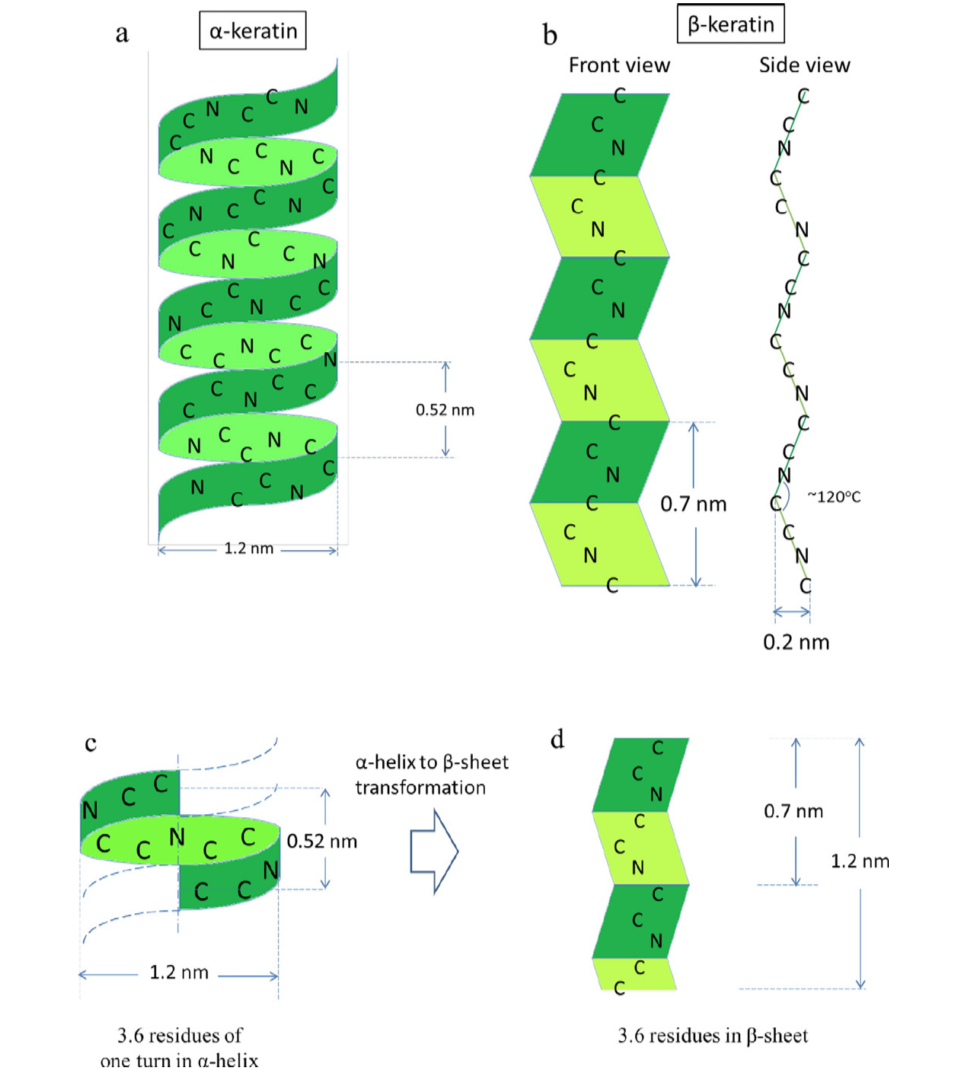
\includegraphics[width=0.55\textwidth]{protein structure.png}
    \caption{protein structure\citep{yu2017structure}}
\end{figure}
but they didn't consider the humidity acting on the chemical bond inside keratin.

Time resolved X-ray scattering experiments on examining keratin structure and a mechanical model are set up in \citep{kreplak2002new}.  Although the result can help us understanding the chemical equillibrium process, still only the environment with a 45\% relative humidity and water is considered.

Besides, Many AFM studies on nanomechanical properties of human hair mainly on cellular structure was done by Bhushan's group in Ohio State University (also structure analasis via SEM and)\citep{bhushan2006afm, seshadri2008situ, wei2005nanomechanical}, and some hair properties about charge, surface protential are done by Kelvin Probe AFM\citep{lodge2007surface, seshadri2008effect}.  All works on hair are summerized here\citep{bhushan2008nanoscale}. 
\begin{figure}[H]
    \centering
    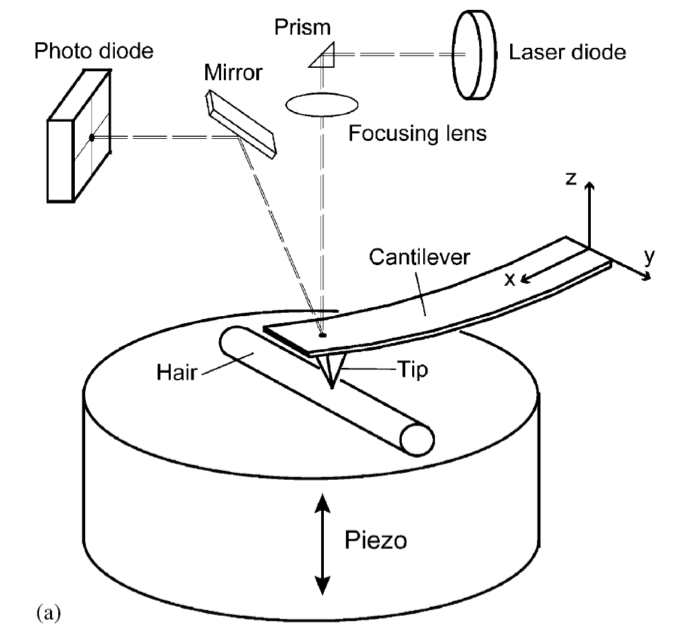
\includegraphics[width=0.36\textwidth]{bhushan.png}
    \caption{AFM method for measuring hair's longitudinal section properties }
\end{figure}
Bhushan's group measured the YM of hair under different humidity and as expected there is a YM decrease with humidity increase. ?? However, this work is not about the relation between hair and keratin. 

\begin{figure}[H]
    \centering
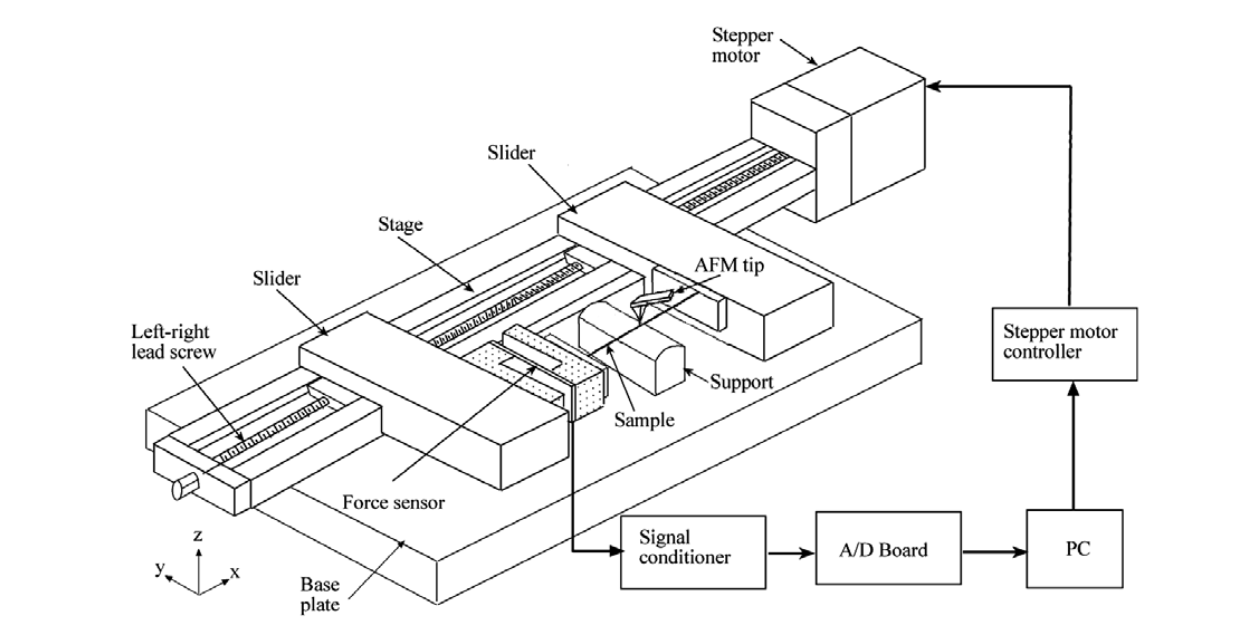
\includegraphics[width=0.7\textwidth]{in situ tensile afm.png}
    \caption{AFM in situ tensile testing of human hair\citep{seshadri2008situ}}
\end{figure} 
They also studied how hair deforms under a certain stress in situ\citep{seshadri2008situ}. They focusing on the surface detail and properties(e.g. $\alpha$-kerotin changes to $\beta$-kerotin) under large strain which we don't care, but at least one result proved that hair deforms following Hooke's Law under small stress(e.g. hair-hydrometer).
\begin{figure}[H]
    \centering
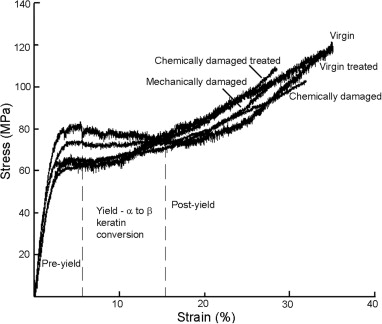
\includegraphics[width=0.6\textwidth]{stress strain.jpg}
    \caption{stress vs strain, you can see at very beginning it appears linear property (Hooke's Law)\citep{seshadri2008situ}}
\end{figure} 
Anyway, the AFM platforms for different test they designed are exquisite and  worth learning.


Simulation and mesoscopic experiments are done in \citep{chou2015mechanics}. They stretch the fiber sample and applied a coarse-grained model to fit.  But not under different environment.

Since there are numerous physical models and explanations, the first thing to do is focusing on the second problem. Then we can develop the solution to the third and the first, which is the core.


\section{Design}
\subsection{Modeling}
\begin{itemize}
    \item 
\end{itemize}

\subsection{Instrumentation}
\textbf{Specimen}: different kerotin fibrils, hairs\\ 
\textbf{AFM}: AFM, T-shaped cantilever with normal tip, oblong cantilever\\
Environment control: Humidity\&Temperature control box (using raspberry and electronic hydrometer\&thermometer to feedback), covering the whole AFM head.

\subsection{Method}
First, we measure the keratin protein's YM under different humidity and temperature.

Second, measure how keratin effect hair's YM (i.e. by control variables only related to keratin inside hair, like using special enzyme(keratinase solution from the culture of feather-degrading bacteria which can 'digest' the keratin and thus to process the hair)\citep{lin1992purification}).  Third, set up the keratin-hair mechanical model, comparing to known model and do the simulation.


\textbf{Notice}: we need to bias the humidity influence on adhesion between tip and specimen.

\subsection{Difficulties and problems}
\begin{itemize}
	    \item How to measure the axial Young's modulus of a nano fiber? If we use nano-strech How to fix an end of kerotin fiber to the base and another to the AFM tip?\\

   \textbf{Possible Solution:}  If we can not find a 	method to fix an end of kerotin fiber, 
				\begin{itemize}
						\item We can measure the transverse YM of keratin using nanoidentation, as long as we know the Poisson ratio, we know the axial YM. However, maybe the Poisson ratio can only accessed from the literature and we can only regard it as a constant which causes final YM unpresise. Besides, the deformation of keratin may differ from transverse nanoindentation  to axial nano-strech.
				\end{itemize}
             
    
    \item How to develop a better hair mechanical model? There must be other relevant factors.

	\item How to control variates? like How to only destroying the protein fibrils inside the hair?


\end{itemize}


\section{Expected Result}
Expected to have quantitatively
\begin{itemize}
	
	\item  a decreased keroin YM with increasing humidity and temparature.
	\item  a precise mechanical model for keratin fibrils
	 \item a proportional relationship between kerotin fibrils YM and hair YM (longitudinal). 
\end{itemize}
\subsection{Expected Finishing Time}
4 weeks. 2 weeks of experiment and 2 weeks for simulation/modeling.

\bibliographystyle{plain}
\bibliography{references}
\end{document}

@article{lee2016advances,
  title={Advances in AFM imaging applications for characterizing the biophysical properties of amyloid fibrils},
  author={Lee, Wonseok and Lee, Hyungbeen and Lee, Gyudo and Yoon, Dae Sung},
  journal={Exploring new findings on amyloidosis},
  year={2016},
  publisher={In Tech, Rijeka}
}

@article{yu2017structure,
  title={Structure and mechanical behavior of human hair},
  author={Yu, Yang and Yang, Wen and Wang, Bin and Meyers, Marc Andr{\'e}},
  journal={Materials Science and Engineering: C},
  volume={73},
  pages={152--163},
  year={2017},
  publisher={Elsevier}
}

@article{Whipple_1921,
	doi = {10.1088/1478-7814/34/1/312},
	url = {https://doi.org/10.1088%2F1478-7814%2F34%2F1%2F312},
	year = 1921,
	month = {dec},
	publisher = {{IOP} Publishing},
	volume = {34},
	number = {1},
	pages = {i--v},
	author = {F J W Whipple},
	title = {The theory of the hair hygrometer},
	journal = {Proceedings of the Physical Society of London},
	abstract = {}
}

@article{bhushan2006afm,
  title={AFM studies of environmental effects on nanomechanical properties and cellular structure of human hair},
  author={Bhushan, Bharat and Chen, Nianhuan},
  journal={Ultramicroscopy},
  volume={106},
  number={8-9},
  pages={755--764},
  year={2006},
  publisher={Elsevier}
}

@article{bhushan2008nanoscale,
  title={Nanoscale characterization of human hair and hair conditioners},
  author={Bhushan, Bharat},
  journal={Progress in Materials Science},
  volume={53},
  number={4},
  pages={585--710},
  year={2008},
  publisher={Elsevier}
}


@article{seshadri2008situ,
  title={In situ tensile deformation characterization of human hair with atomic force microscopy},
  author={Seshadri, Indira P and Bhushan, Bharat},
  journal={Acta Materialia},
  volume={56},
  number={4},
  pages={774--781},
  year={2008},
  publisher={Elsevier}
}

@article{wei2005nanomechanical,
  title={Nanomechanical characterization of human hair using nanoindentation and SEM},
  author={Wei, Guohua and Bhushan, Bharat and Torgerson, Peter M},
  journal={Ultramicroscopy},
  volume={105},
  number={1-4},
  pages={248--266},
  year={2005},
  publisher={Elsevier}
}

@article{lodge2007surface,
  title={Surface potential measurement of human hair using Kelvin probe microscopy},
  author={Lodge, Richard A and Bhushan, Bharat},
  journal={Journal of Vacuum Science \& Technology A: Vacuum, Surfaces, and Films},
  volume={25},
  number={4},
  pages={893--902},
  year={2007},
  publisher={AVS}
}

@article{seshadri2008effect,
  title={Effect of rubbing load on nanoscale charging characteristics of human hair characterized by AFM based Kelvin probe},
  author={Seshadri, Indira P and Bhushan, Bharat},
  journal={Journal of colloid and interface science},
  volume={325},
  number={2},
  pages={580--587},
  year={2008},
  publisher={Elsevier}
}

@article{chou2015mechanics,
  title={Mechanics of trichocyte alpha-keratin fibers: Experiment, theory, and simulation},
  author={Chou, Chia-Ching and Lepore, Emiliano and Antonaci, Paola and Pugno, Nicola and Buehler, Markus J},
  journal={Journal of Materials Research},
  volume={30},
  number={1},
  pages={26--35},
  year={2015},
  publisher={Cambridge University Press}
}

@article{kreplak2002new,
  title={A new deformation model of hard $\alpha$-keratin fibers at the nanometer scale: implications for hard $\alpha$-keratin intermediate filament mechanical properties},
  author={Kreplak, L and Franbourg, A and Briki, F and Leroy, F and Dalle, D and Doucet, J},
  journal={Biophysical journal},
  volume={82},
  number={4},
  pages={2265--2274},
  year={2002},
  publisher={Elsevier}
}

@article{lin1992purification,
  title={Purification and characterization of a keratinase from a feather-degrading Bacillus licheniformis strain},
  author={Lin, Xiang and Lee, Chung-Ginn and Casale, Ellen S and Shih, Jason CH},
  journal={Appl. Environ. Microbiol.},
  volume={58},
  number={10},
  pages={3271--3275},
  year={1992},
  publisher={Am Soc Microbiol}
}

